\chapter{PRÉSENTATION ET IMPLÉMENTATION DE LA SOLUTION}

\section{Introduction}
\label{sec:intro-ddqn}

Ce chapitre présente la conception et l'implémentation d'un agent d'apprentissage par renforcement basé sur l'algorithme \gls{ddqn} (\textit{Double Deep Q-Network}) pour l'optimisation des transmissions LR-FHSS. Nous détaillons la formulation du problème en tant que processus de décision markovien, l'architecture du réseau de neurones, l'environnement d'entraînement et l'algorithme d'apprentissage.

\section{Problématique et formalisme MDP}
\label{sec:problematique-mdp}
Notre travail vise à assurer la fiabilité et l'efficacité énergétique des transmissions dans les réseaux LoRaWAN utilisant LR-FHSS. Nous proposons pour cela une approche basée sur l'apprentissage par renforcement profond (DRL), où un agent intelligent, situé sur un serveur de bordure, apprend une politique de transmission optimale à travers son interaction avec l'environnement.

\subsection{Formulation en processus de décision markovien}
\label{subsec:formulation-mdp}

Le problème d'optimisation des transmissions LR-FHSS peut être formulé comme un \gls{mdp} (\textit{Markov Decision Process}). Un MDP est un cadre mathématique pour modéliser la prise de décision séquentielle dans un environnement où les résultats sont en partie aléatoires et en partie sous le contrôle de l'agent. Il est formellement défini par le tuple $(\mathcal{S}, \mathcal{A}, \mathcal{P}, \mathcal{R}, \gamma)$ \cite{puterman1994mdp,sutton2018reinforcement} :

\begin{itemize}
	\item \textbf{$\mathcal{S}$ : L'espace d'états}. Il représente l'ensemble des informations pertinentes dont dispose l'agent au moment de prendre une décision. Dans notre cas, l'état capture la situation d'un nœud avant une transmission.
	
	\item \textbf{$\mathcal{A}$ : L'espace d'actions}. Il s'agit de l'ensemble des choix discrets disponibles pour l'agent. Ici, une action correspond à la sélection simultanée d'un débit de données et d'une puissance d'émission.
	
	\item \textbf{$\mathcal{P}(s' \mid s, a)$ : La dynamique de transition}. C'est la probabilité de passer de l'état $s$ à l'état $s'$ après avoir exécuté l'action $a$. Cette dynamique est régie par l'environnement (le simulateur) et est inconnue de l'agent.
	
	\item \textbf{$\mathcal{R}(s, a, s')$ : La fonction de récompense}. C'est un signal scalaire immédiat qui évalue la qualité de la transition de l'état $s$ à l'état $s'$ suite à l'action $a$. L'objectif de l'agent est de maximiser la somme de ces récompenses sur le long terme.
	
	\item \textbf{$\gamma \in [0, 1]$ : Le facteur d'actualisation (\textit{discount factor})}. Il détermine l'importance accordée aux récompenses futures par rapport aux récompenses immédiates. Un $\gamma$ proche de 1 rend l'agent ``prévoyant'', tandis qu'un $\gamma$ proche de 0 le rend ``court-termiste''.
\end{itemize}

L'objectif de l'agent est de trouver une politique $\pi^* : \mathcal{S} \rightarrow \mathcal{A}$ qui maximise l'espérance de la somme actualisée des récompenses futures :

\begin{equation}
	\pi^* = \arg\max_{\pi} \mathbb{E}_{\tau \sim \pi} \left[ \sum_{t=0}^{\infty} \gamma^t r_t \right]
\end{equation}

où $\tau = (s_0, a_0, r_0, s_1, a_1, r_1, \ldots)$ est une trajectoire (ou épisode) générée en suivant la politique $\pi$.

\subsection{\texorpdfstring{Définition de l'espace d'états $\mathcal{S}$}{Définition de l'espace d'états}}
\label{subsec:espace-etats}

L'état $s_t \in \mathbb{R}^8$ est un vecteur de huit variables normalisées, conçu pour fournir à l'agent une représentation concise mais complète de la situation d'un nœud avant une transmission. Chaque composante est choisie pour son influence sur la décision optimale.

\begin{figure}[H]
	\centering
	\begin{tikzpicture}[node distance=1.1cm, auto, >=latex]
		% --- Colonne de GAUCHE ---
		\node[rectangle, draw, fill=blue!10, minimum width=2.8cm, minimum height=0.7cm] (d_norm) {$d_{\text{norm}}$};
		\node[rectangle, draw, fill=blue!10, minimum width=2.8cm, minimum height=0.7cm, below of=d_norm] (snr_avg) {$\text{SNR}_{\text{avg}}$};
		\node[rectangle, draw, fill=blue!10, minimum width=2.8cm, minimum height=0.7cm, below of=snr_avg] (tau_success) {$\tau_{\text{success}}$};
		\node[rectangle, draw, fill=blue!10, minimum width=2.8cm, minimum height=0.7cm, below of=tau_success] (r_norm) {$r_{\text{norm}}$};
		
		% --- Colonne de DROITE ---
		\node[rectangle, draw, fill=blue!10, minimum width=2.8cm, minimum height=0.7cm, right=4cm of d_norm] (log_d) {$\log(d)_{\text{norm}}$};
		\node[rectangle, draw, fill=blue!10, minimum width=2.8cm, minimum height=0.7cm, below of=log_d] (t_day) {$t_{\text{day}}$};
		\node[rectangle, draw, fill=blue!10, minimum width=2.8cm, minimum height=0.7cm, below of=t_day] (sigma_snr) {$\sigma_{\text{SNR}}$};
		\node[rectangle, draw, fill=blue!10, minimum width=2.8cm, minimum height=0.7cm, below of=sigma_snr] (l_norm) {$L_{\text{norm}}$};
		
		% --- Point de jonction au milieu ---
		% On définit un point invisible au centre des deux colonnes
		\coordinate (center) at ($(r_norm.south)!0.5!(l_norm.south) + (0,-1)$);
		
		% --- Bloc ÉTAT (en bas au centre) ---
		\node[rectangle, draw, fill=green!10, minimum width=6cm, minimum height=1cm, below=1.5cm of center] (state) {État $s_t \in \mathbb{R}^8$};
		
		% --- Lignes GAUCHE (partent du côté gauche, contournent et rejoignent le centre) ---
		\foreach \i in {d_norm, snr_avg, tau_success, r_norm} {
			\draw[thick] (\i.west) -- ++(-0.5,0) |- (center);
		}
		
		% --- Lignes DROITE (partent du côté droit, contournent et rejoignent le centre) ---
		\foreach \i in {log_d, t_day, sigma_snr, l_norm} {
			\draw[thick] (\i.east) -- ++(0.5,0) |- (center);
		}
		
		% --- Flèche finale vers le vecteur d'état ---
		\draw[->, thick] (center) -- (state.north);
		
	\end{tikzpicture}
	\caption{Composition de l'espace d'états $\mathcal{S}$.}
	\label{fig:etat-vecteur}
\end{figure}

Le tableau~\ref{tab:state-space-ddqn} détaille chaque composante, sa plage de valeurs et sa justification.

\begin{table}[!ht]
	\centering
	\caption{Description détaillée des composantes de l'espace d'états.}
	\label{tab:state-space-ddqn}
	\begin{tabular}{|p{2.5cm}|p{2cm}|p{8cm}|}
		\hline
		\textbf{Variable} & \textbf{Plage} & \textbf{Description et justification} \\
		\hline
		$d_{\text{norm}}$ & [0, 1] & Distance à la passerelle normalisée par la portée maximale. La distance est le principal facteur influençant l'atténuation du signal. \\
		\hline
		$\text{SNR}_{\text{avg}}$ & [-1, 1] & Moyenne du SNR (\textit{Signal-to-Noise Ratio}) des trois dernières transmissions. Normalisée par une valeur typique de 20 dB. Indicateur direct de la qualité récente du lien. \\
		\hline
		$\tau_{\text{success}}$ & [0, 1] & Taux de succès des cinq dernières transmissions. Permet à l'agent d'ajuster sa stratégie en fonction de la performance récente. \\
		\hline
		$r_{\text{norm}}$ & [0, 1] & Nombre de retransmissions consécutives après un échec, normalisé par 5. Un nombre élevé indique des conditions de canal dégradées et doit inciter à une configuration plus robuste. \\
		\hline
		$\log(d)_{\text{norm}}$ & [0, 1] & Logarithme de la distance normalisé. L'atténuation du signal étant proportionnelle à $\log(d)$, cette transformation linéarise la relation et facilite l'apprentissage. \\
		\hline
		$t_{\text{day}}$ & [0, 1] & Variable de phase temporelle, prévue pour modéliser des variations diurnes du canal (activité humaine, interférences variables). Dans le cadre de cette étude, les simulations couvrent des durées inférieures à 24h et aucune variation temporelle du canal n'est implémentée ; cette composante reste donc constante et constitue une extension pour les travaux futurs.  \\
		\hline
		$\sigma_{\text{SNR}}$ & [0, 1] & Stabilité du signal, définie comme l'inverse de l'écart-type des trois derniers SNR. Un canal stable (valeur proche de 1) permet d'utiliser des configurations plus agressives. \\
		\hline
		$L_{\text{norm}}$ & [0, 1] & Taille de la charge utile (payload) en octets, normalisée par la taille maximale autorisée (123 octets). Influence directement le temps d'antenne (ToA) et donc le risque de collision. \\
		\hline
	\end{tabular}
\end{table}

La normalisation de toutes les composantes dans des plages bornées ($[0, 1]$ ou $[-1, 1]$) est essentielle pour stabiliser l'apprentissage du réseau de neurones. Elle évite que des variables avec de grandes amplitudes numériques ne dominent le processus de mise à jour des poids.

\subsection{\texorpdfstring{Définition de l'espace d'actions $\mathcal{A}$}{Définition de l'espace d'actions}}
\label{subsec:espace-actions}

L'espace d'actions $\mathcal{A}$ est un espace discret. Une action $a \in \mathcal{A}$ correspond à la sélection simultanée d'un DR et d'une puissance d'émission :

\begin{equation}
	\mathcal{A} = \underbrace{\{\text{DR}8, \text{DR}9, \text{DR}10, \text{DR}11\}}_{4 \text{ DR}} \times \underbrace{\{-4, -3, \dots, 13, 14\}}_{19 \text{ puissances}}
\end{equation}

Le nombre total d'actions est donc $|\mathcal{A}| = 4 \times 19 = 76$. Chaque action est encodée par un entier unique $a \in \{0, 1, \dots, 75\}$. Cet espace d'action discret est parfaitement adapté à l'algorithme \gls{dqn} et à ses dérivés. Il capture l'ensemble des configurations de transmission valides pour la bande EU868.

\subsection{Conception de la fonction de récompense}
\label{subsec:fonction-recompense}

La fonction de récompense est l'élément le plus critique de la formulation du \gls{mdp}. Elle traduit les objectifs de notre approche (fiabilité, efficacité énergétique et efficacité spectrale) en un signal d'apprentissage concret. Nous proposons une structure paramétrée permettant d'équilibrer ces objectifs souvent contradictoires par l'ajustement de coefficients de pondération.

La récompense totale $\mathcal{R}$ est définie de manière conditionnelle selon l'issue de la transmission :

\begin{equation}
	\mathcal{R} = 
	\begin{cases} 
		\phi & \text{si échec} \\
		\rho + \mathcal{R}_{\text{ToA}} + \mathcal{R}_{\text{power}} + \mathcal{R}_{\text{retry}} + \Omega(\text{SNR}, \text{DR}) & \text{si succès}
	\end{cases}
\end{equation}

Les composantes de cette fonction sont définies comme suit :

\begin{itemize}
	\item \textbf{Base de performance ($\phi, \rho$)} : 
	Le paramètre $\phi$ pénalise l'échec pour garantir la fiabilité, tandis que $\rho$ est la récompense de base pour un succès.
	\[ \phi = -200, \quad \rho = +100 \]
	Ces valeurs soulignent que l'échec est deux fois plus coûteux que le succès n'est gratifiant, forçant l'agent à privilégier la délivrance du paquet.
	
	\item \textbf{Pénalité d'occupation spectrale ($\mathcal{R}_{\text{ToA}}$)} :
	Elle pénalise le temps d'occupation du canal (temps d'antenne) normalisé par le ToA maximum théorique ($T_{max} = 3813.376$ ms).
	\begin{equation}
		\mathcal{R}_{\text{ToA}} = -\alpha \cdot \min\left(\frac{\text{ToA}_{\text{ms}}}{T_{max}}, 1\right) \quad \text{avec } \alpha = 80
	\end{equation}
	Cette pénalité encourage l'agent à minimiser la durée de ses transmissions, réduisant ainsi les risques de collision et améliorant l'efficacité énergétique et spectrale globale du réseau.
	
	\item \textbf{Pénalité d'efficacité énergétique ($\mathcal{R}_{\text{power}}$)} : 
	Elle sanctionne l'utilisation de puissances d'émission élevées sur la plage normalisée du matériel (ici de -4 à 14 dBm).
	\begin{equation}
		\mathcal{R}_{\text{power}} = -\beta \cdot \left( \frac{P_{\text{TX}} + 4}{18} \right) \quad \text{avec } \beta = 50
	\end{equation}
	
	\item \textbf{Pénalité de retransmission ($\mathcal{R}_{\text{retry}}$)} : 
	Elle incite l'agent à minimiser le nombre de tentatives ($N_{retry}$) pour réduire la congestion.
	\begin{equation}
		\mathcal{R}_{\text{retry}} = -\gamma \cdot (\frac{N_{retry}}{5}) \quad \text{avec } \gamma = 30
	\end{equation}
	
	\item \textbf{Optimisation de la qualité du lien ($\Omega$)} : 
	Ce terme regroupe les bonus de robustesse ($\mathcal{R}_{\text{SNR}}$) et d'efficacité spectrale ($\mathcal{R}_{\text{DR}}$) :
	
	\[ \mathcal{R}_{\text{SNR}} = 
	\begin{cases} 
		+\delta & \text{si } -5 \leq \text{SNR} \leq 5 \text{ dB (Optimal)} \\
		-\epsilon \cdot \max(0, \text{SNR} - 10) & \text{si } \text{SNR} > 10 \text{ dB (Overkill)} \\
		0 & \text{sinon}
	\end{cases} \]
	
	Avec $\delta = 20$ et $\epsilon = 4$. La zone de SNR ``optimale'' est définie comme une marge suffisante pour garantir la réception sans excès.
	
	\item \textbf{Bonus d'efficacité spectrale ($\mathcal{R}_{\text{DR}}$)} : Il favorise l'utilisation de \gls{dr} plus efficaces (ceux avec un \gls{cr} de 2/3) lorsque les conditions de canal le permettent.
	\begin{equation}
		\mathcal{R}_{\text{DR}} =
		\begin{cases}
			0 & \text{si DR} = 8 \\
			+10 & \text{si DR} = 9 \\
			+5 & \text{si DR} = 10 \\
			+15 & \text{si DR} = 11
		\end{cases}
	\end{equation}
\end{itemize}


L'utilisation de ces paramètres ($\alpha, \beta, \gamma, \delta, \epsilon$) permet de séparer la logique de décision de l'agent (stratégie LR-FHSS) des valeurs numériques concrètes. Cette séparation facilite l'ajustement et l'optimisation ultérieure de la politique de l'agent via des méthodes de recherche d'hyperparamètres, sans modifier la structure de la fonction de récompense elle-même.


\subsubsection{Analyse des poids relatifs des objectifs de la fonction de récompense}
\label{subsec:poids-relatifs-objectifs}

L'analyse des poids relatifs permet de quantifier l'importance de chaque objectif dans le processus d'apprentissage de l'agent. Les calculs sont basés sur les plages de variation de chaque composante.



\begin{table}[H]
	\centering
	\caption{Poids relatifs individuels des composantes de la récompense}
	\label{tab:poids-individuels}
	\begin{tabular}{|l|c|c|c|c|}
		\hline
		\textbf{Composante} & \textbf{Symbole} & \textbf{Plage} & \textbf{Poids absolu} & \textbf{Poids relatif} \\
		\hline
		Échec / Succès & $\phi, \rho$ & $[-200, +100]$ & 300 & 53,27\% \\
		\hline
		Retransmissions & $\gamma$ & $[-30, 0]$ & 30 & 5,33\% \\
		\hline
		Qualité du lien (SNR) & $\delta, \epsilon$ & $[-80, +20]$ & 100 & 17,76\% \\
		\hline
		Temps d'occupation (ToA) & $\alpha$ & $[-80, -11,82]$ & 68,18 & 12,10\% \\
		\hline
		Puissance d'émission & $\beta$ & $[-50, 0]$ & 50 & 8,88\% \\
		\hline
		Efficacité spectrale (DR) & — & $[0, +15]$ & 15 & 2,66\% \\
		\hline
		\textbf{TOTAL} & & & \textbf{563,18} & \textbf{100\%} \\
		\hline
	\end{tabular}
\end{table}

L’analyse des poids attribués aux différentes composantes de la fonction de récompense permet d’identifier clairement les priorités de l’agent :

\begin{enumerate}
	\item \textbf{Garantir la fiabilité des transmissions} :
	Le critère succès/échec représente à lui seul un poids de 53,27\%. En intégrant également la pénalité liée aux retransmissions, cette proportion atteint 58,6\%. Cela indique que l’objectif principal de l’agent consiste à maximiser le taux de transmissions réussies tout en limitant les retransmissions.
	
	\item \textbf{Optimiser l’efficacité spectrale et énergétique} :
	Le cumul des métriques associées à ces performances représente 41,4\% du poids total, constituant ainsi le second objectif majeur après la fiabilité. Par ailleurs, en tenant compte de l’impact indirect des retransmissions sur la consommation énergétique à long terme, cette valeur atteint 46,76\%.
\end{enumerate}


\section{Architecture de l'agent DDQN}
\label{sec:architecture-agent-ddqn}
Cette section décrit l’architecture de l’agent DDQN. Elle présente d’abord le principe de l’algorithme Double Deep Q-Network (DDQN) et les améliorations par rapport au DQN classique, puis détaille l’architecture du réseau de neurones qui implémente cet agent.

\subsection{Principe de l'algorithme DDQN}
\label{subsec:principe-ddqn}

L'algorithme \gls{ddqn} est une amélioration du \gls{dqn} (\textit{Deep Q-Network}) original \cite{mnih2015dqn,vanhasselt2016ddqn}, conçu pour résoudre le problème de surestimation systématique des valeurs $Q$ dans le DQN. Ce biais est lié à l'utilisation de l'opérateur \textit{$\max$} dans la mise à jour de la cible.

Dans le \gls{dqn} standard, la valeur cible pour la mise à jour est calculée comme suit :
\begin{equation}
	y_t^{\text{DQN}} = r_t + \gamma \max_{a'} Q_{\theta^-}(s_{t+1}, a')
\end{equation}
où :
\begin{itemize}
	\item $y_t^{\text{DQN}}$ est la valeur cible utilisée pour entraîner le réseau principal ;
	\item $r_t$ est la récompense immédiate reçue après avoir pris l'action $a_t$ dans l'état $s_t$ ;
	\item $\gamma$ est le facteur d'actualisation (\textit{discount factor}) qui pondère l'importance des récompenses futures ;
	\item $s_{t+1}$ est l'état suivant observé après l'action ;
	\item $a'$ représente toutes les actions possibles dans l'état $s_{t+1}$ ;
	\item $Q_{\theta^-}$ est le réseau cible (\textit{target network}), une copie gelée périodiquement du réseau principal $Q_\theta$.
\end{itemize}
Le problème avec le \gls{dqn} classique est que le même réseau est utilisé à la fois pour sélectionner et évaluer l'action, ce qui propage les erreurs d'estimation et conduit à des valeurs $Q$ trop optimistes.

Le \gls{ddqn} propose une solution en découplant la sélection de l'action de son évaluation :
\begin{equation}
	y_t^{\text{DDQN}} = r_t + \gamma Q_{\theta^-}\left(s_{t+1}, \arg\max_{a'} Q_\theta(s_{t+1}, a')\right)
\end{equation}
où :
\begin{itemize}
	\item $y_t^{\text{DDQN}}$ est la nouvelle valeur cible pour le Double DQN ;
	\item $\arg\max_{a'} Q_\theta(s_{t+1}, a')$ désigne l'action qui maximise la valeur Q selon le réseau principal $Q_\theta$ ;
	\item $Q_{\theta^-}(s_{t+1}, \cdot)$ évalue cette action sélectionnée à l'aide du réseau cible.
\end{itemize}
Cette séparation permet de réduire le biais de surestimation et d'obtenir un apprentissage plus stable.

\begin{figure}[!h]
	\centering
	\begin{subfigure}{0.8\textwidth}
		\centering
		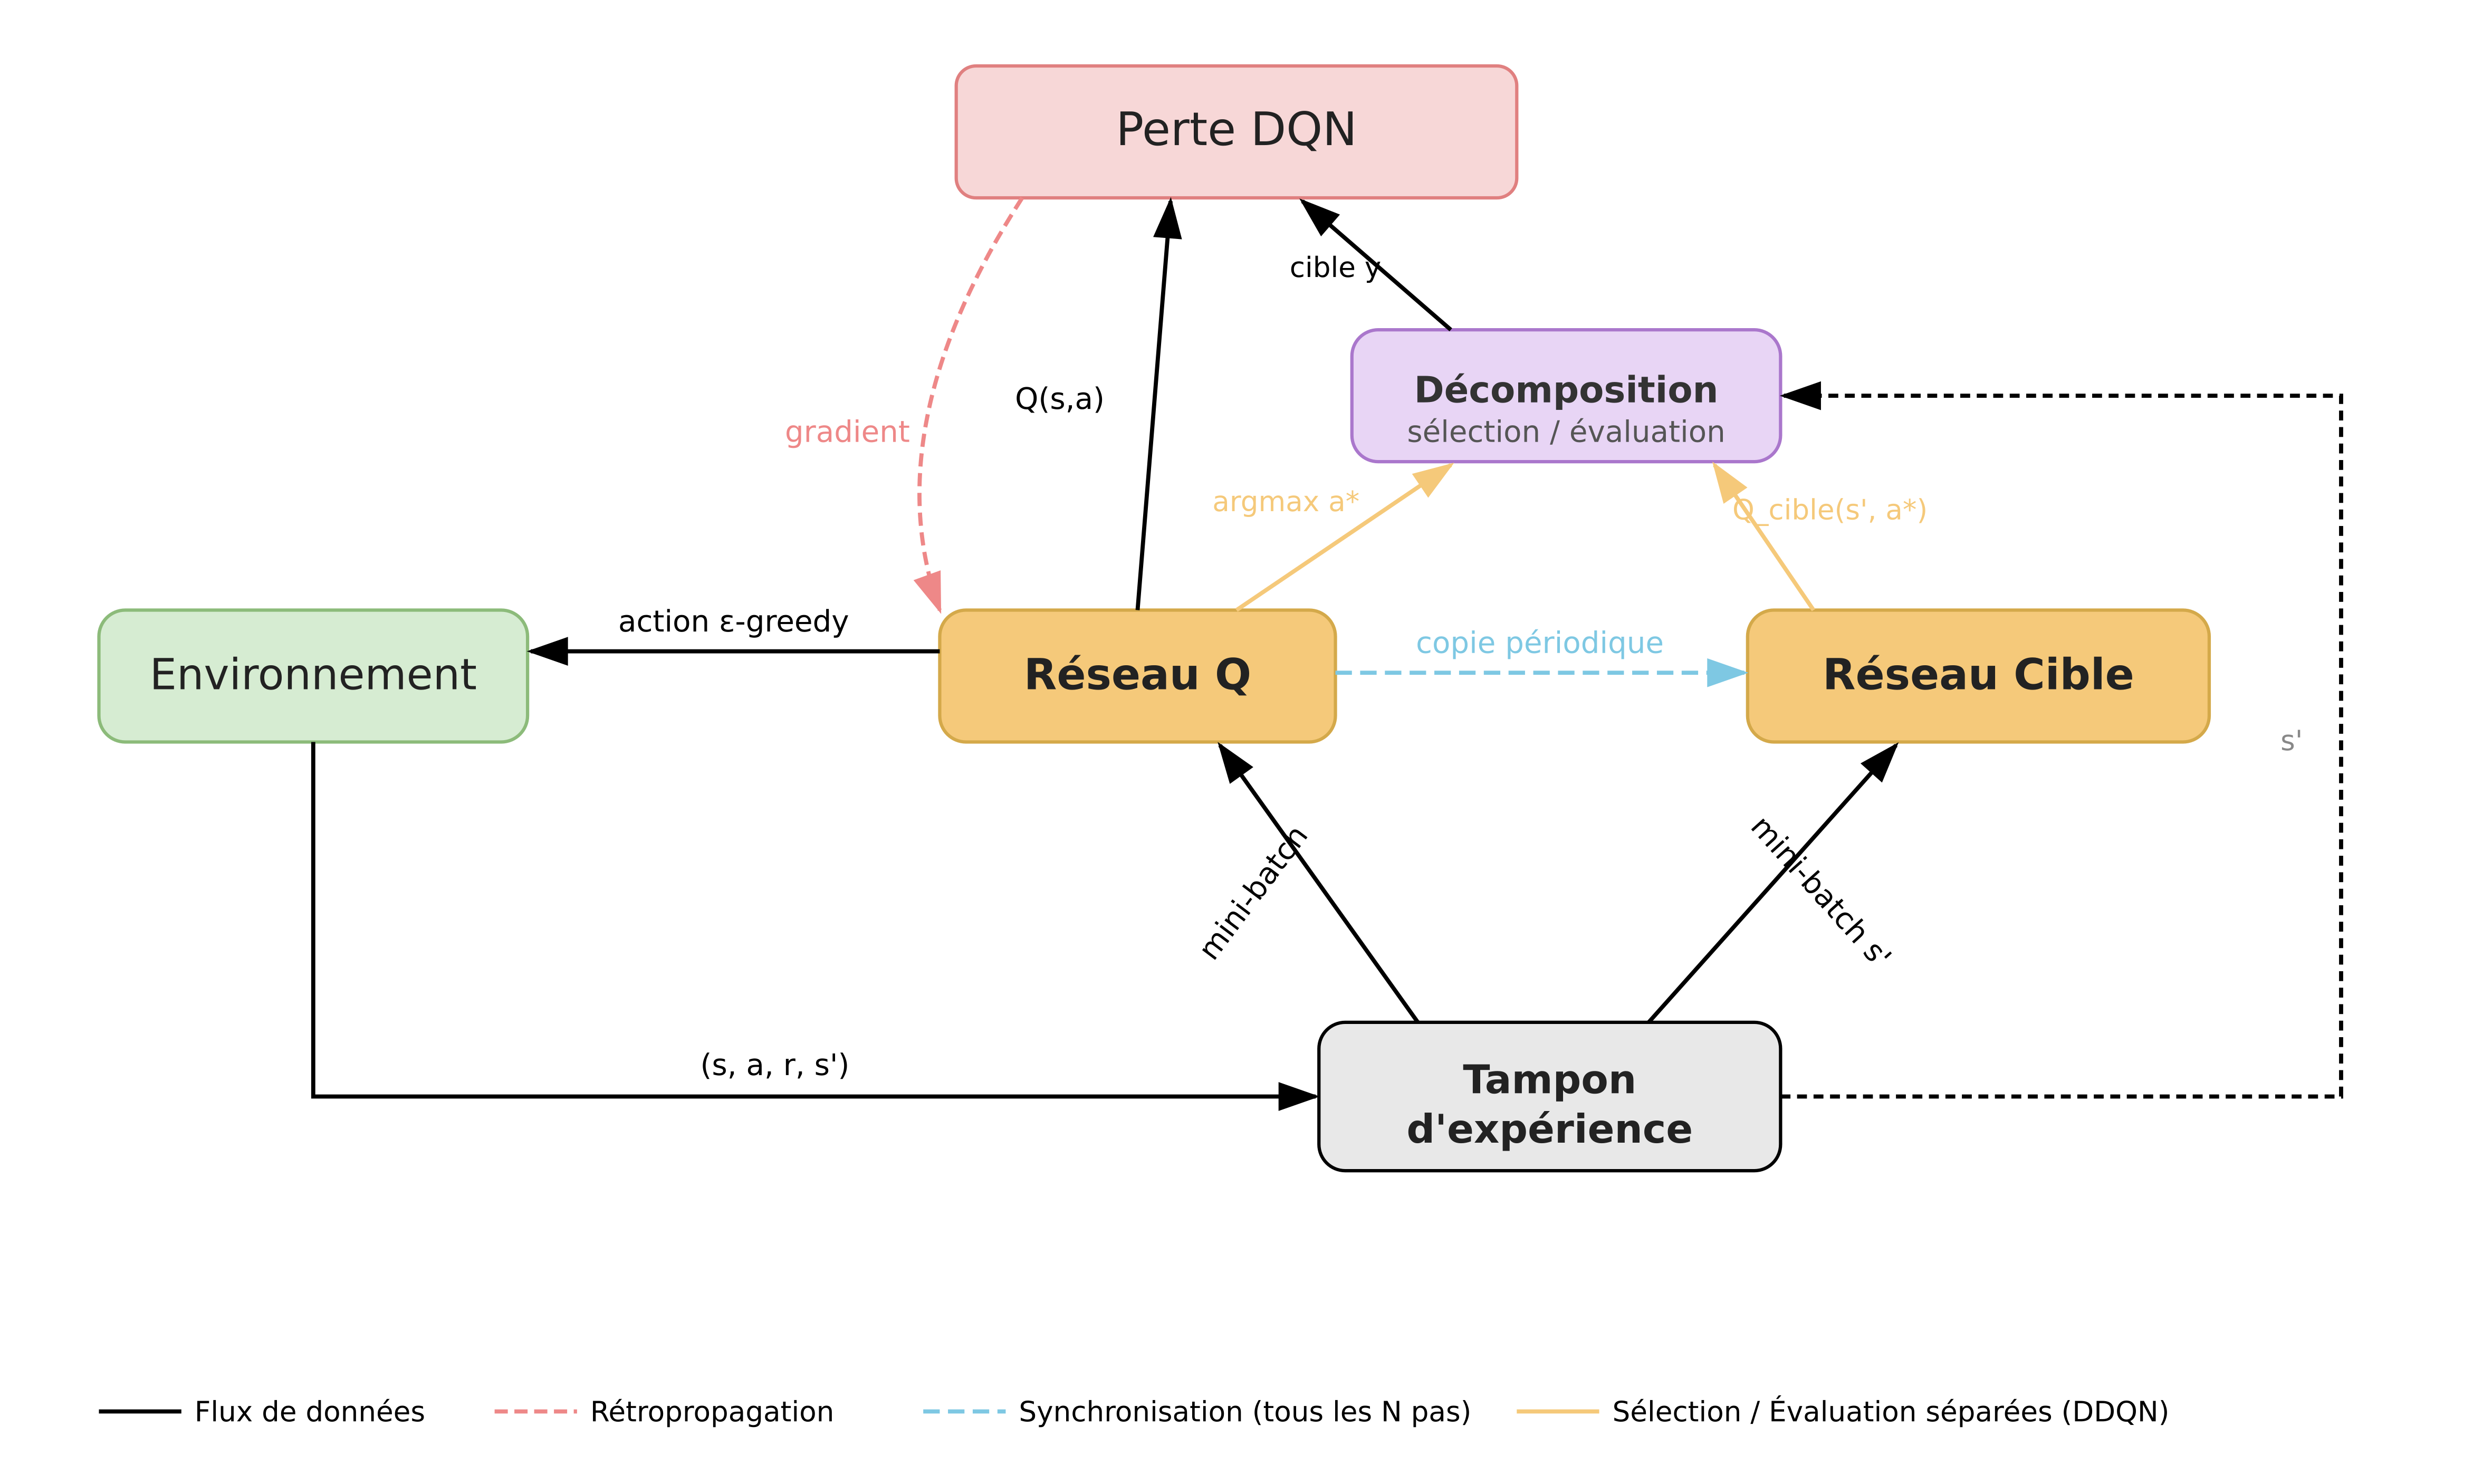
\includegraphics[width=\textwidth]{images/ddqn_architecture.png}
		\caption{Architecture DDQN}
		\label{fig:ddqn}
	\end{subfigure}
	\hfill
	\begin{subfigure}{0.8\textwidth}
		\centering
		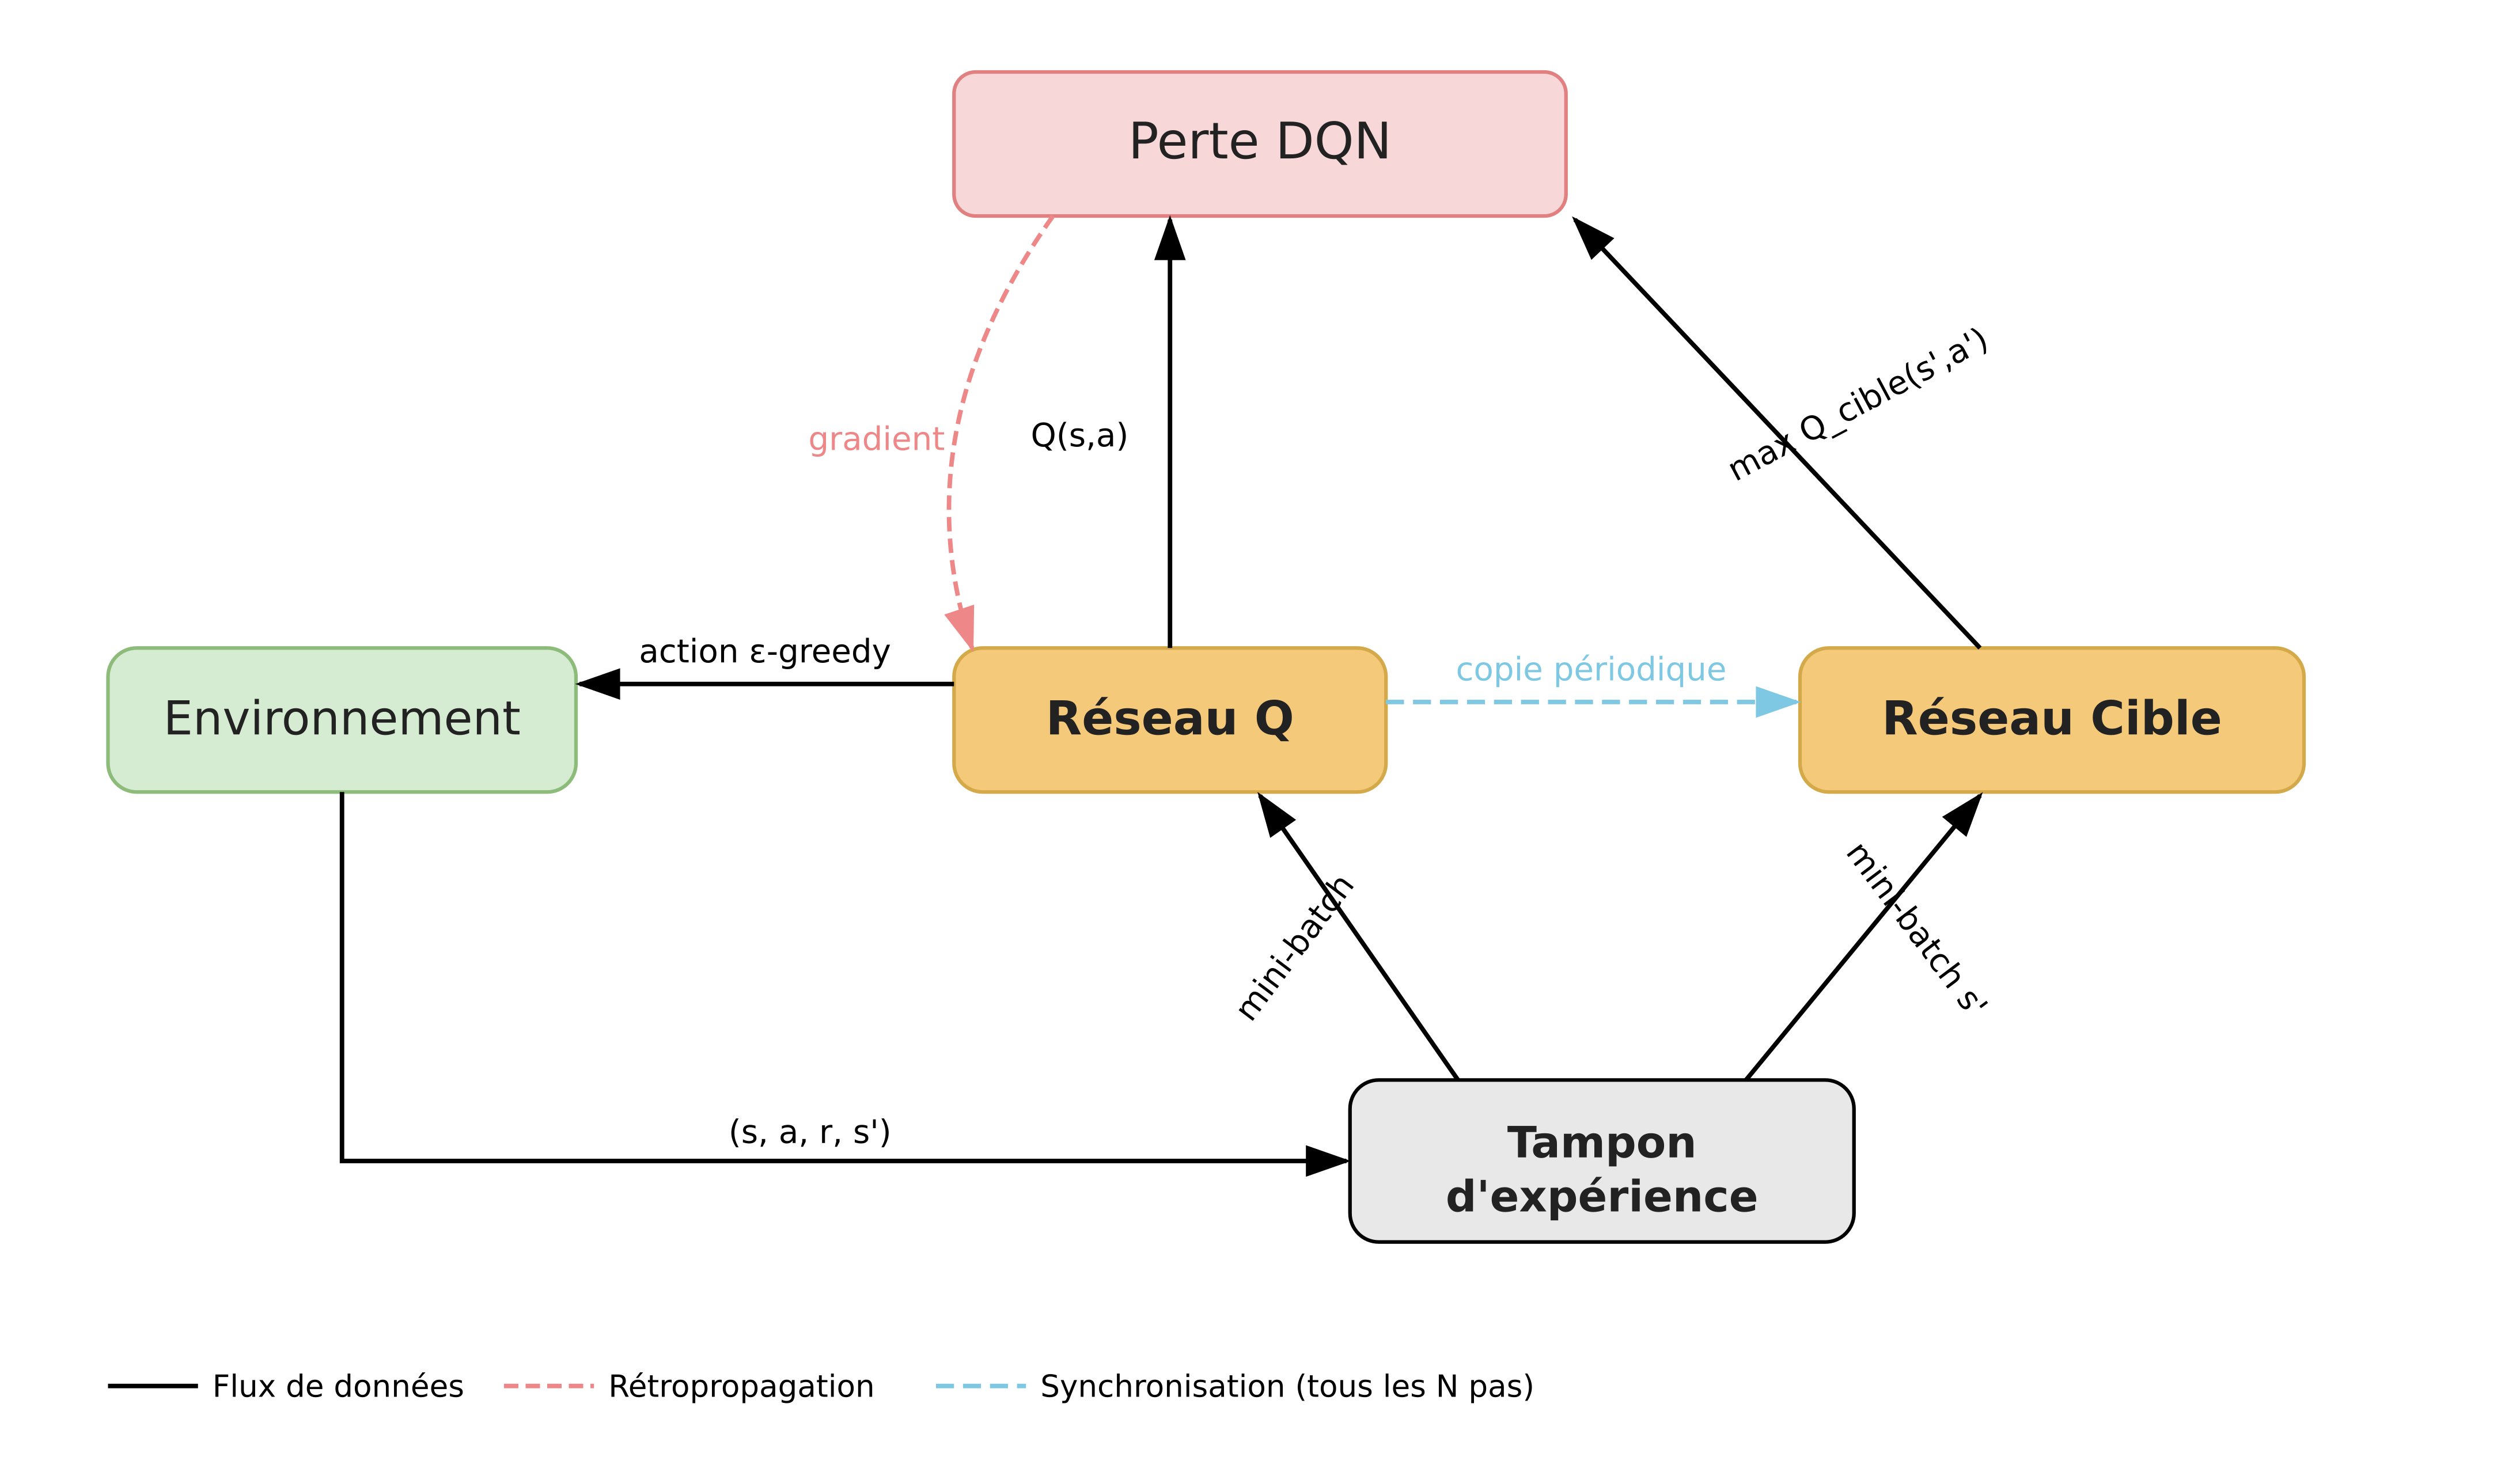
\includegraphics[width=\textwidth]{images/dqn_architecture.png}
		\caption{Architecture DQN}
		\label{fig:dqn}
	\end{subfigure}
	\caption{Comparaison des architectures DQN et DDQN}
	\label{fig:comparaison}
\end{figure}

Cette double estimation, où le réseau principal sélectionne la meilleure action et le réseau cible l'évalue, réduit significativement le biais de surestimation et améliore la stabilité et la rapidité de la convergence.

\clearpage
\subsection{Architecture du réseau de neurones}
\label{subsec:architecture-reseau}

L'architecture repose sur un réseau de neurones multi-couches de type feedforward, conformément à l'approche introduite par \cite{mnih2015dqn}. Celui-ci est composé de deux couches cachées entièrement connectées (128 et 64 neurones) avec fonction d'activation ReLU, choisie pour ses propriétés de convergence rapide et sa capacité à atténuer le problème du gradient évanescent \cite{nair2010relu}. 

Afin de limiter le sur-apprentissage et d'améliorer la capacité de généralisation du modèle, une régularisation par Dropout avec un taux de 0,1 est appliquée après la première couche cachée, suivant la méthodologie proposée par \cite{srivastava2014dropout}. 

La couche de sortie comporte 76 neurones linéaires correspondant aux valeurs $Q(s,a)$ pour chaque action possible. Aucune fonction d'activation n'est utilisée en sortie, conformément à la formulation du Deep Q-Network où les valeurs Q ne sont pas bornées \cite{mnih2015dqn}. 

Les fondements théoriques de l'approximation de fonction en apprentissage par renforcement s'appuient également sur les travaux de référence de \cite{sutton2018rl}.

\begin{figure}[H]
	\centering
	\resizebox{0.95\textwidth}{!}{%
		\begin{tikzpicture}[
			neuron/.style={circle, draw, minimum size=0.6cm, inner sep=0pt, font=\tiny},
			layer/.style={rectangle, draw, minimum width=1.8cm, minimum height=0.7cm, rounded corners, font=\small},
			arrow/.style={->, >=stealth, thick}
			]
			
			% Couche d'entrée (8 neurones)
			\foreach \i in {1,...,8} {
				\node[neuron, fill=blue!20] (input-\i) at (0, -0.7*\i) {};
			}
			\node[below of=input-8, node distance=0.7cm, font=\small] {Entrée (8)};
			
			% Première couche cachée (128 neurones)
			\node[layer, fill=green!20, right=1.6cm of input-4] (hidden1) {Couche 1};
			\node[below of=hidden1, node distance=0.9cm, font=\tiny] {128 neurones};
			
			% Dropout
			\node[layer, fill=yellow!20, right=1.6cm of hidden1] (dropout) {Dropout};
			\node[below of=dropout, node distance=0.9cm, font=\tiny] {p = 0.1};
			
			% Deuxième couche cachée (64 neurones)
			\node[layer, fill=green!20, right=1.6cm of dropout] (hidden2) {Couche 2};
			\node[below of=hidden2, node distance=0.9cm, font=\tiny] {64 neurones};
			
			% Couche de sortie (76 neurones)
			\node[layer, fill=orange!20, right=1.6cm of hidden2] (output) {Sortie};
			\node[below of=output, node distance=0.9cm, font=\tiny] {76 neurones};
			
			% Connexions
			\draw[arrow] (input-4.east) -- node[above, sloped, font=\tiny] {8→128} (hidden1.west);
			\draw[arrow] (hidden1.east) -- (dropout.west);
			\draw[arrow] (dropout.east) -- (hidden2.west);
			\draw[arrow] (hidden2.east) -- (output.west);
			
		\end{tikzpicture}%
	}
	\caption{Architecture du réseau DDQN.}
	\label{fig:ddqn-architecture}
\end{figure}

L'architecture se compose des éléments suivants :
\begin{enumerate}
	\item \textbf{Couche d'entrée} : 8 neurones, correspondant aux 8 dimensions de l'espace d'états.
	\item \textbf{Première couche cachée} : 128 neurones avec une fonction d'activation ReLU (\textit{Rectified Linear Unit}). Cette couche projette l'état dans un espace de dimension supérieure, permettant de capturer des interactions complexes entre les variables d'entrée.
	\item \textbf{Couche de Dropout} : Une couche de régularisation qui désactive aléatoirement 10\% des neurones de la couche précédente pendant l'entraînement. Cela force le réseau à apprendre des représentations redondantes et réduit le risque de sur-apprentissage.
	\item \textbf{Seconde couche cachée} : 64 neurones avec activation ReLU. Elle compresse l'information apprise en une représentation plus compacte.
	\item \textbf{Couche de sortie} : 76 neurones, chacun correspondant à la valeur $Q(s, a)$ estimée pour une action spécifique. Aucune fonction d'activation n'est appliquée en sortie, car les valeurs $Q$ peuvent être négatives.
\end{enumerate}

Cette architecture contient un peu plus de 14 000 paramètres, ce qui permet une inférence en quelques millisecondes sur un processeur standard, rendant l'agent parfaitement adapté à une utilisation en temps réel.

\section{Algorithme et environnement d'entraînement}
\label{sec:algorithme-entrainement}
Cette section décrit l’algorithme d’entraînement de l’agent DDQN et l’environnement
utilisé pour simuler les transmissions LR-FHSS. Elle présente d’abord l’environnement
d’apprentissage et la stratégie d’exploration, puis détaille les mécanismes clés de
l’apprentissage, l’algorithme complet, et enfin l’analyse des hyperparamètres et
de la convergence.

\subsection{Environnement d'apprentissage}
\label{subsec:environnement-sequentiel}

L'entraînement de l'agent s'effectue dans un environnement dédié, \texttt{TrainingEnvironment}, qui simule des épisodes de transmissions. À chaque épisode, les conditions de départ (distance, ombrage) sont tirées aléatoirement selon une distribution réaliste. Cette diversité de situations force l'agent à apprendre une politique généraliste, applicable à n'importe quel nœud du réseau, plutôt qu'une politique sur-optimisée pour un seul scénario.

\begin{figure}[H]
	\centering
	\begin{tikzpicture}[node distance=1.5cm, auto]
		% Début de l'épisode
		\node[rectangle, draw, fill=blue!10, rounded corners] (reset) {Choix de la distance};
		
		% Boucle temporelle
		\node[rectangle, draw, fill=green!10, rounded corners, below of=reset] (action) {Agent choisit $(DR, P_{TX})$};
		\node[rectangle, draw, fill=yellow!10, rounded corners, below of=action] (transmission) {Simulation transmission};
		\node[rectangle, draw, fill=orange!10, rounded corners, below of=transmission] (reward) {Calcul récompense $\mathcal{R}$};
		\node[rectangle, draw, fill=red!10, rounded corners, below of=reward] (transition) {Transition vers $s_{t+1}$};
		
		% Flèches
		\draw[->, thick] (reset) -- (action);
		\draw[->, thick] (action) -- (transmission);
		\draw[->, thick] (transmission) -- (reward);
		\draw[->, thick] (reward) -- (transition);
		\draw[<-, thick] (action.east) -- ++(1,0) node[right] {Fin épisode?} -- ++(0, -4.5) -| (transition.east);
		
		% Conditions de fin
		\node[rectangle, draw, fill=gray!10, dashed, right=2cm of transition] (end) {Si $t \geq T_{\max}$};
		
	\end{tikzpicture}
	\caption{Déroulement d'un épisode dans l'environnement d'entraînement.}
	\label{fig:training-episode}
\end{figure}

Le modèle de propagation et les calculs de \gls{rssi}, \gls{snr}, \gls{ber} ainsi que l'évaluation de la réussite ou de l'échec de la transmission sont assurés par notre simulateur calibré sur l'étude de référence \cite{lrfhss_comparaison}.

\subsection{\texorpdfstring{Stratégie d'exploration : $\epsilon$-greedy}{Stratégie d'exploration : epsilon-greedy}}
\label{subsec:epsilon-greedy}

Pendant l'entraînement, l'agent doit équilibrer deux phases contradictoires : l'exploration, où il essaie de nouvelles actions pour découvrir leurs conséquences, et l'exploitation, où il utilise ses connaissances actuelles pour maximiser la récompense. La stratégie $\epsilon$-greedy est une méthode simple et efficace pour gérer ce compromis.

Avec une probabilité $\epsilon$, l'agent choisit une action aléatoirement (exploration). Avec une probabilité $1-\epsilon$, il choisit l'action qui maximise la valeur $Q$ estimée pour l'état courant (exploitation).

\begin{equation}
	a_t =
	\begin{cases}
		\text{action aléatoire uniforme} & \text{avec probabilité } \epsilon_t \\
		\arg\max_{a} Q_\theta(s_t, a) & \text{avec probabilité } 1 - \epsilon_t
	\end{cases}
\end{equation}

Le paramètre $\epsilon$ n'est pas constant. Il suit une décroissance exponentielle dans le temps :
\begin{equation}
	\epsilon_t = \max(\epsilon_{\text{min}}, \epsilon_{\text{start}} \times \epsilon_{\text{decay}}^t)
\end{equation}
La figure suivante  \ref{fig:epsilon-decay-3000} illustre cette évolution.

\begin{figure}[H]
	\centering
	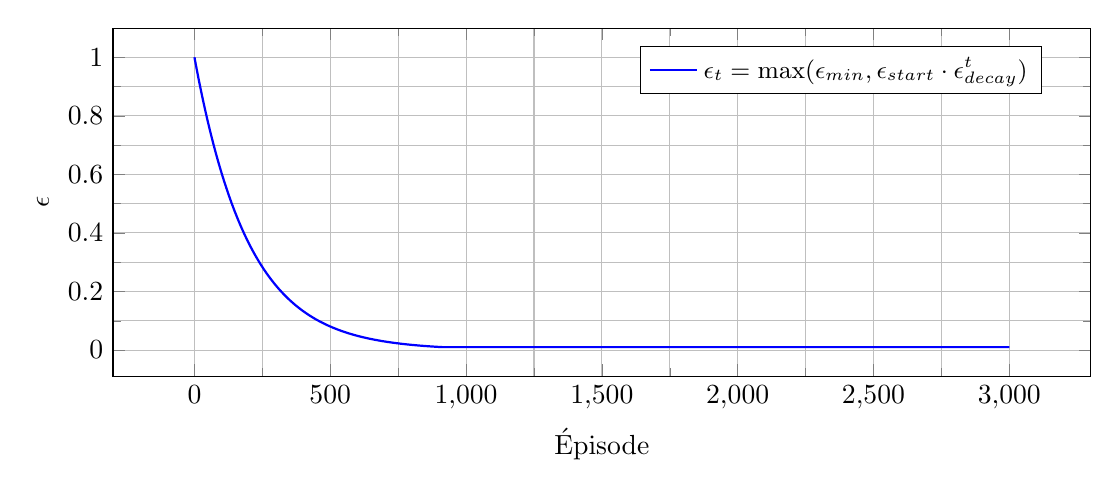
\begin{tikzpicture}
		\begin{axis}[
			width=14cm, height=6cm,
			xlabel={Épisode},
			ylabel={$\epsilon$},
			grid=both,
			minor tick num=1,
			xtick={0,500,1000,1500,2000,2500,3000},
			ytick={0,0.2,0.4,0.6,0.8,1.0},
			domain=0:3000,
			samples=1000,
			legend style={at={(0.95,0.95)}, anchor=north east, font=\small},
			]
			\addplot[blue, thick] {max(0.01, 1.0 * 0.995^x)};
			\addlegendentry{$\epsilon_t = \max(\epsilon_\text{min}, \epsilon_\text{start} \cdot \epsilon_\text{decay}^t)$}
		\end{axis}
	\end{tikzpicture}
	
	\caption{Évolution du paramètre d'exploration $\epsilon$.}
	\label{fig:epsilon-decay-3000}
\end{figure}

Cette décroissance permet à l'agent d'explorer largement les actions possibles au début, puis de se concentrer progressivement sur l'affinage de la politique apprise.

\subsection{Mécanismes clés de l'apprentissage}
\label{subsec:mecanismes-apprentissage}
Cette sous-section décrit les principaux mécanismes utilisés pour stabiliser et améliorer l’apprentissage de l’agent DDQN. Elle présente d’abord la mémoire d’expérience (Replay Buffer) qui permet de stocker et réutiliser les transitions, puis le rôle des réseaux principal et cible pour assurer une mise à jour stable des valeurs Q.

\subsubsection{Mémoire d’expérience (Replay Buffer)}
L'agent utilise une mémoire d’expérience, notée $\mathcal{D}$, pour stocker ses expériences passées. Chaque expérience est une transition $(s_t, a_t, r_t, s_{t+1}, d_t)$, où $d_t$ indique si l'épisode est terminé. Pendant l'entraînement, l'agent échantillonne aléatoirement un mini-lot (\textit{batch}) de transitions depuis cette mémoire pour mettre à jour son réseau.

Ce mécanisme présente deux avantages majeurs :
\begin{enumerate}
	\item Il brise la corrélation temporelle entre les expériences consécutives, ce qui stabilise l'apprentissage.
	\item Il permet de réutiliser des expériences rares ou anciennes, améliorant l'efficacité d'échantillonnage.
\end{enumerate}

\subsubsection{Réseaux cible et principal}
L'agent maintient deux réseaux de neurones distincts :
\begin{itemize}
	\item Le \textbf{réseau principal} $Q_\theta$, qui est mis à jour à chaque étape par descente de gradient pour minimiser l'erreur de prédiction.
	\item Le \textbf{réseau cible} $Q_{\theta^-}$, qui est une copie du réseau principal mise à jour plus lentement. Il est utilisé pour calculer la valeur cible $y_t$, stabilisant ainsi l'apprentissage.
\end{itemize}

La mise à jour du réseau cible se fait par une mise a jour lente (\textit{soft update}) :
\begin{equation}
	\theta^- \leftarrow \tau \theta + (1 - \tau) \theta^-
\end{equation}
avec $\tau \ll 1$ (typiquement 0,005). Cette mise à jour progressive évite les changements brusques de la cible.

\subsection{Algorithme d'entraînement complet}
\label{subsec:algo-complet}

L'algorithme~\ref{alg:ddqn-training} synthétise l'ensemble du processus d'entraînement de l'agent DDQN.

\begin{algorithm}[H]
	\caption{Entraînement de l'agent DDQN pour l'optimisation LR-FHSS}
	\label{alg:ddqn-training}
	\begin{algorithmic}[1]
		\Require Environnement d'entraînement $E$, nombre d'épisodes $N$
		\Ensure Réseau principal $Q_\theta$ (politique apprise)
		
		\State Initialiser le réseau principal $Q_\theta$ avec des poids aléatoires
		\State Initialiser le réseau cible $Q_{\theta^-}$ avec les mêmes poids que $Q_\theta$
		\State Initialiser la mémoire de replay $\mathcal{D}$ (capacité $C = 10 000$)
		\State Initialiser le paramètre d'exploration $\epsilon \leftarrow 1.0$
		
		\For{épisode $e = 1$ à $N$}
		\State $s \gets E.\text{reset}()$ \Comment{Nouvel épisode, nouvel état initial}
		\State $R_{\text{total}} \gets 0$
		
		\While{l'épisode n'est pas terminé}
		\State $a \gets$ sélectionner action avec $\epsilon$-greedy à partir de $Q_\theta(s)$
		\State $(r, s', d) \gets E.\text{step}(a)$ \Comment{Exécuter l'action dans l'environnement}
		\State Stocker $(s, a, r, s', d)$ dans $\mathcal{D}$
		\State $R_{\text{total}} \gets R_{\text{total}} + r$
		
		\If{$|\mathcal{D}| \geq$ batch\_size}
		\State Échantillonner un mini-lot $\mathcal{B}$ de transitions depuis $\mathcal{D}$
		\State Calculer les valeurs cibles $y$ pour chaque transition de $\mathcal{B}$ (équation DDQN)
		\State Mettre à jour $Q_\theta$ par descente de gradient sur la perte $\mathcal{L} = \frac{1}{|\mathcal{B}|}\sum (Q_\theta(s,a) - y)^2$
		\State Mettre à jour le réseau cible : $\theta^- \leftarrow \tau \theta + (1 - \tau) \theta^-$
		\EndIf
		
		\State $s \gets s'$
		\EndWhile
		
		\State $\epsilon \gets \max(\epsilon_{\text{min}}, \epsilon \times \epsilon_{\text{decay}})$
		\State Journaliser les métriques de l'épisode ($R_{\text{total}}$, taux de succès, etc.)
		\EndFor
		
		\State \Return $Q_\theta$
	\end{algorithmic}
\end{algorithm}

\subsection{Hyperparamètres et courbes d'apprentissage}
Cette sous-section présente d’abord la configuration des hyperparamètres utilisés pour l’entraînement de l’agent DDQN, puis analyse la convergence du modèle à travers les courbes de récompense, de taux de succès et de perte, illustrant la stabilité et l’efficacité de l’apprentissage.
\subsubsection{Configuration des hyperparamètres}
Le tableau suivant présente les hyperparamètres utilisés pour l'entraînement de notre modèle DDQN.
\begin{table}[H] 
	\centering
	\caption{Hyperparamètres de l'apprentissage DDQN}
	\label{tab:hyperparameters}
	\begin{tabular}{|l|c|l|}
		\hline
		\textbf{Hyperparamètre} & \textbf{Valeur} & \textbf{Description} \\
		\hline
		\multicolumn{3}{|c|}{\textbf{Paramètres du réseau}} \\
		\hline
		Taux d'apprentissage ($\alpha$) & $10^{-4}$ & Pas de mise à jour du réseau \\
		Facteur d'actualisation ($\gamma$) & 0,99 & Importance des récompenses futures \\
		Taille du batch & 64 & Nombre d'expériences par apprentissage \\
		\hline
		\multicolumn{3}{|c|}{\textbf{Mémoire et exploration}} \\
		\hline
		Taille du replay buffer & 10 000 & Capacité maximale de mémoire \\
		$\epsilon_{initial}$ & 1 & Probabilité d'exploration initiale \\
		$\epsilon_{final}$ & 0,05 & Probabilité d'exploration minimale \\
		Décroissance d'$\epsilon$ & 0,995 & Facteur de réduction par épisode \\
		\hline
		\multicolumn{3}{|c|}{\textbf{Synchronisation}} \\
		\hline
		Fréquence mise à jour cible & 100 pas & Pas entre synchronisations \\
		$\tau$ (soft update) & 0,001 & Taux de mise à jour progressive \\
		\hline
		\multicolumn{3}{|c|}{\textbf{Environnement}} \\
		\hline
		Nombre d'épisodes & 3000 & Durée totale d'entraînement \\
		Pas par épisode & 100 & Interactions par épisode \\
		\hline
	\end{tabular}
\end{table}	

\subsubsection{Analyse de la convergence}

La figure \ref{fig:reward} illustre la progression de l'apprentissage avec une forte variance initiale (épisodes 1-100) où les récompenses fluctuent entre -12431 et +6979, caractéristique d'une phase d'exploration intensive visible dans la figure \ref{fig:epsilon}. Une convergence progressive s'opère à partir de 450 épisodes, avec une récompense moyenne stabilisée autour de 6870 ± 2150 sur les 500 derniers épisodes.

Le taux de succès (Fig. \ref{fig:success}) atteint 89\% en moyenne en fin d'entraînement, avec des pics réguliers à 100\% dès l'épisode 6 et des séquences soutenues de réussite complète (notamment aux épisodes 920-935), démontrant l'efficacité de l'approche proposée.

L'évolution de la fonction de perte (Fig. \ref{fig:loss}) confirme un apprentissage stable du réseau : après une augmentation initiale traduisant l'acquisition des connaissances, la perte se stabilise autour de 198 ± 8 à partir de 1000 épisodes, indiquant une convergence satisfaisante.

\begin{figure}[H]
	\centering
	\begin{subfigure}[b]{0.48\textwidth}
		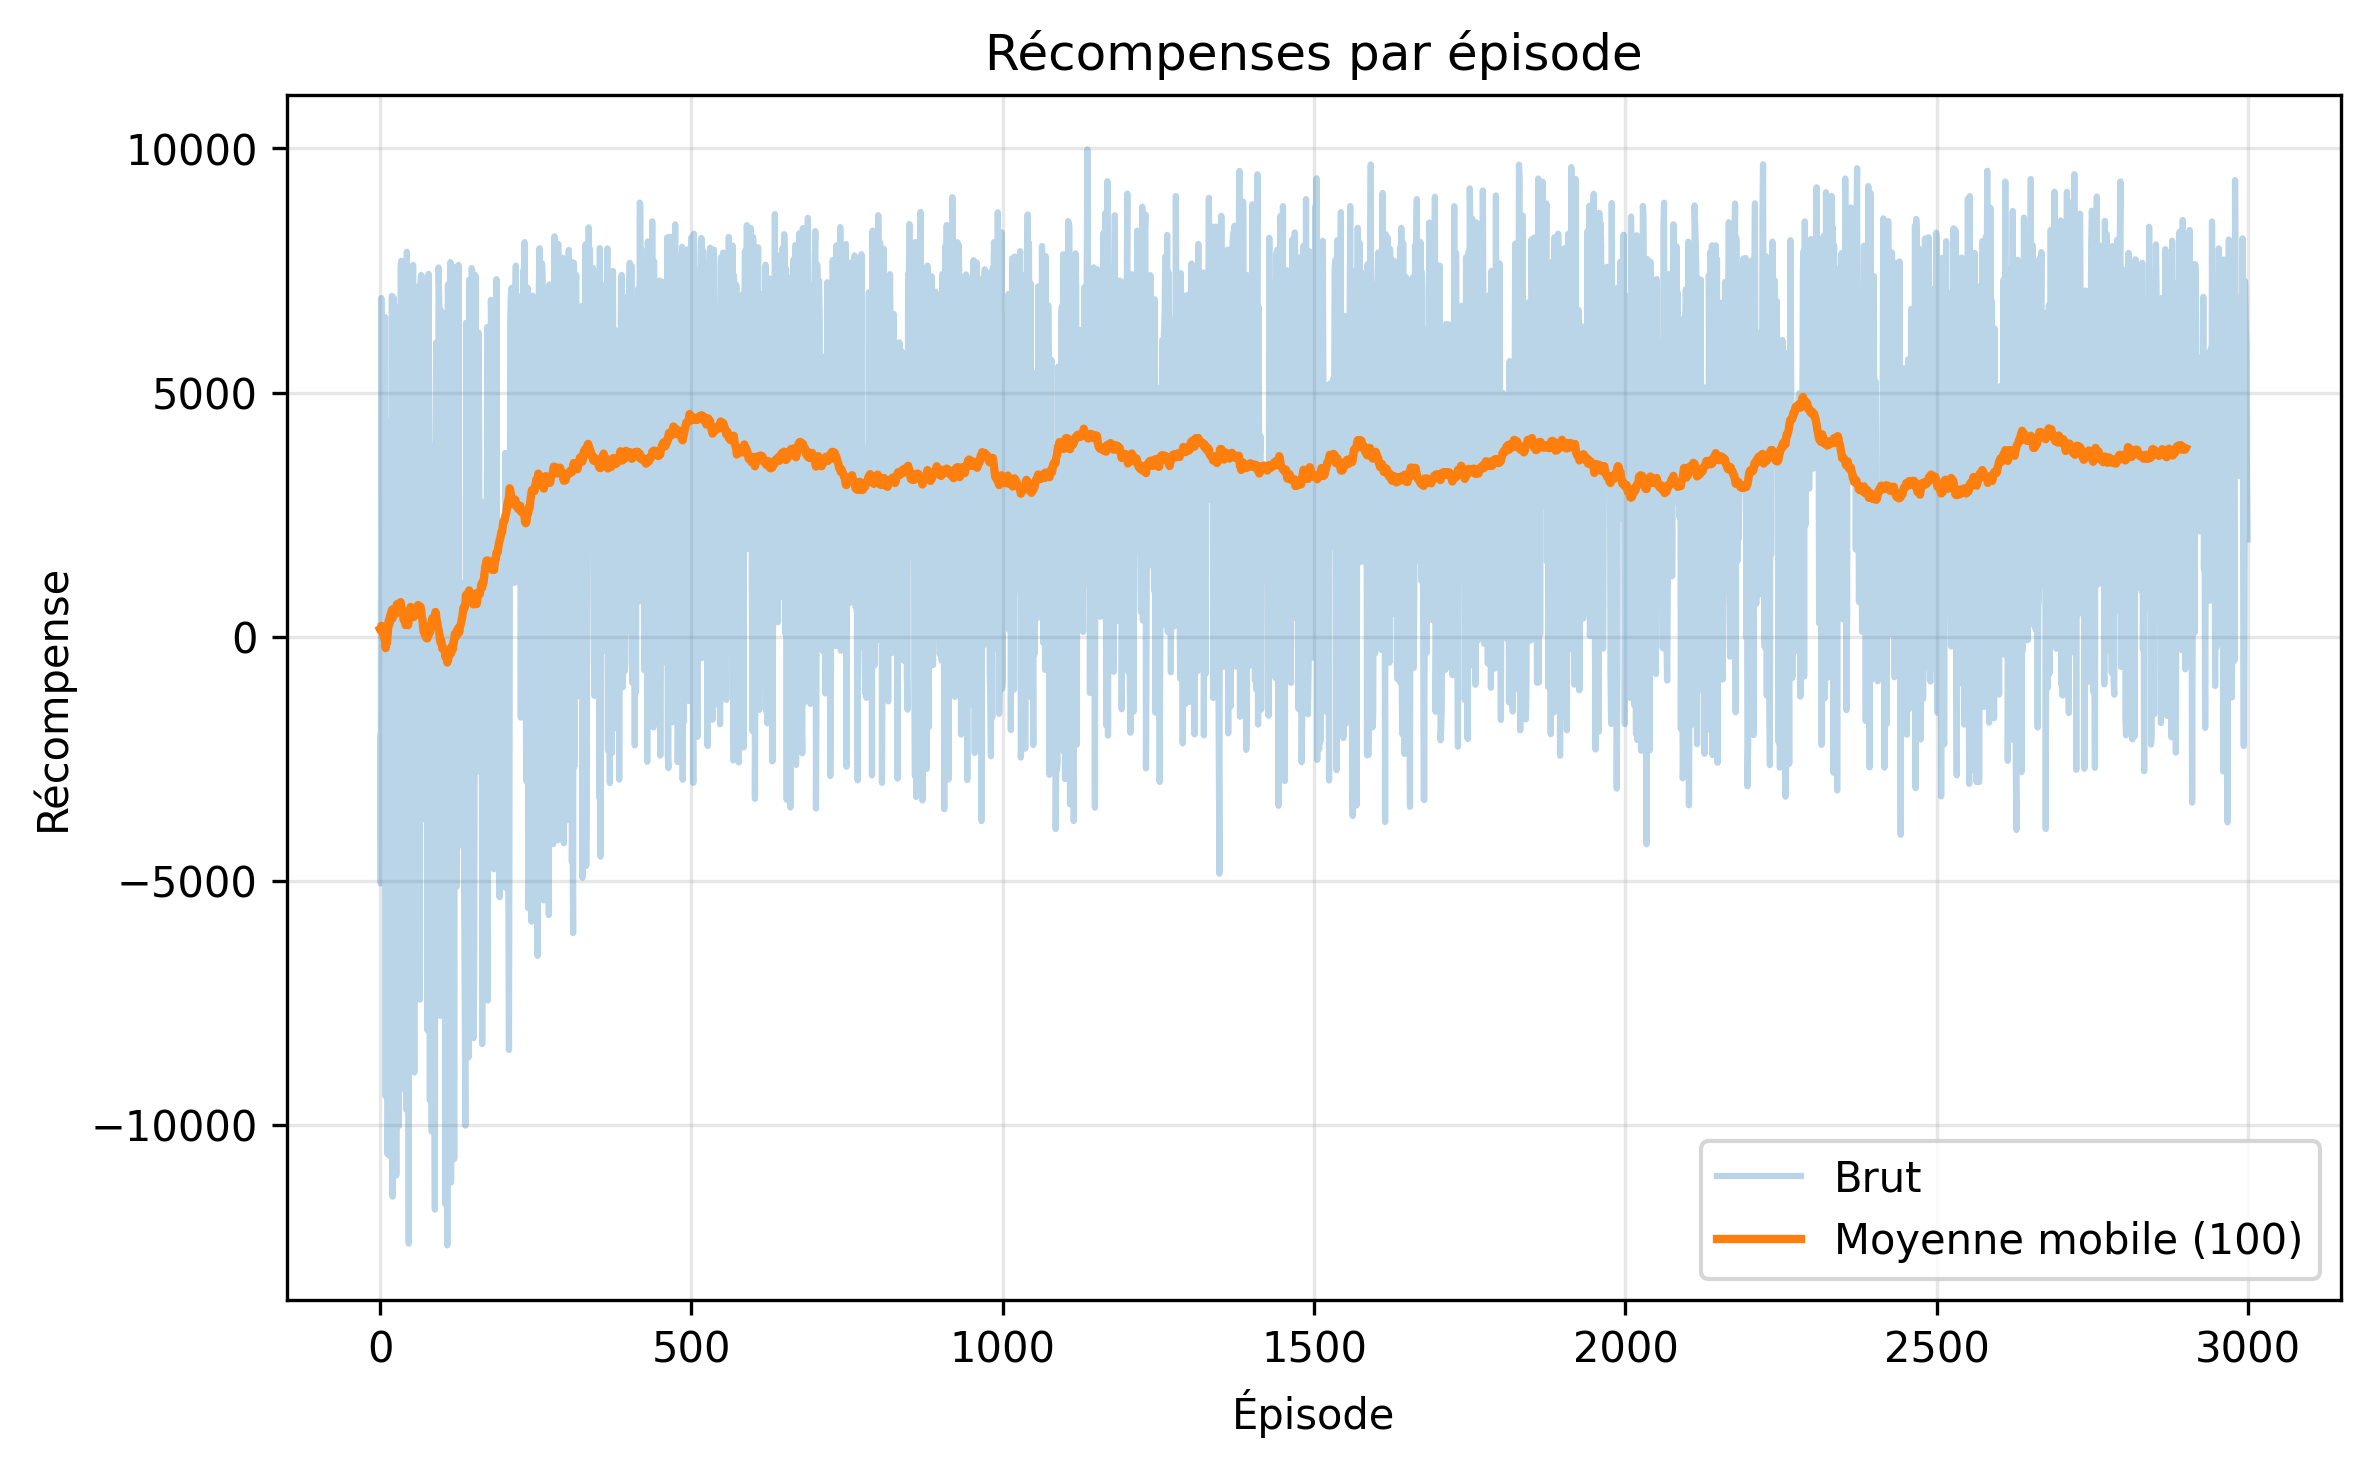
\includegraphics[width=\textwidth]{images/validation/training/01_recompenses.png}
		\caption{Récompense cumulée par épisode}
		\label{fig:reward}
	\end{subfigure}
	\hfill
	\begin{subfigure}[b]{0.48\textwidth}
		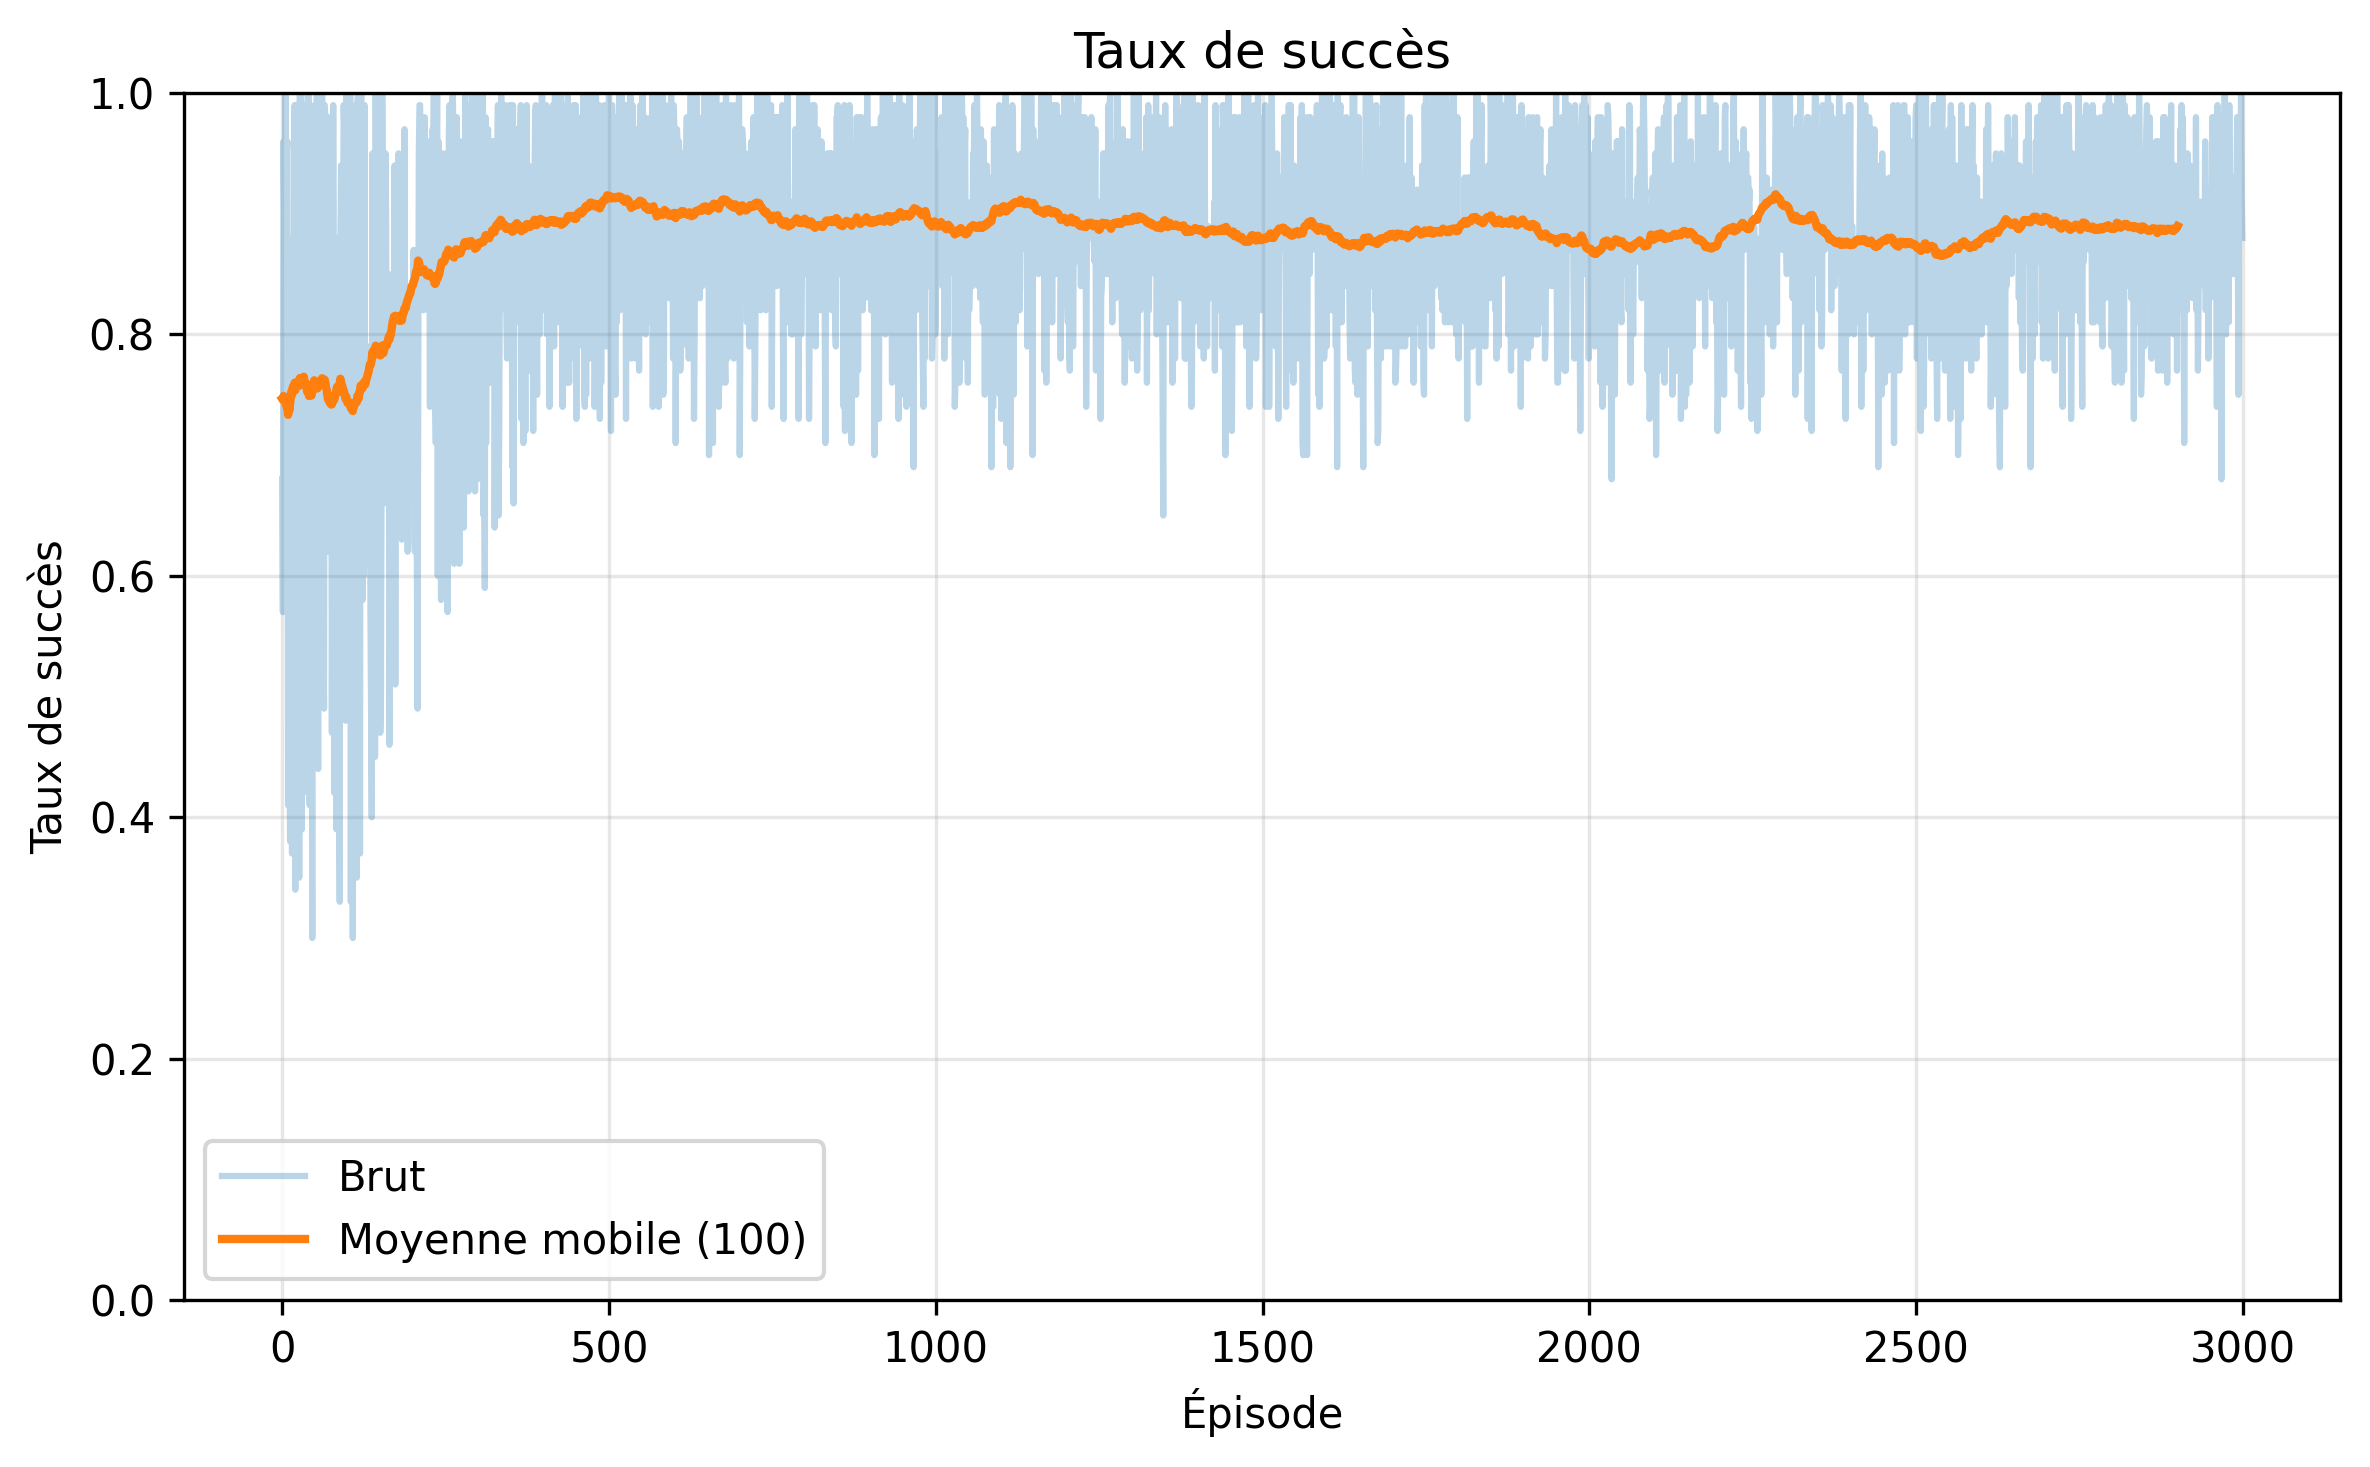
\includegraphics[width=\textwidth]{images/validation/training/02_taux_succes.png}
		\caption{Taux de succès des paquets}
		\label{fig:success}
	\end{subfigure}
	
	\vspace{0.3cm}
	
	\begin{subfigure}[b]{0.48\textwidth} 
		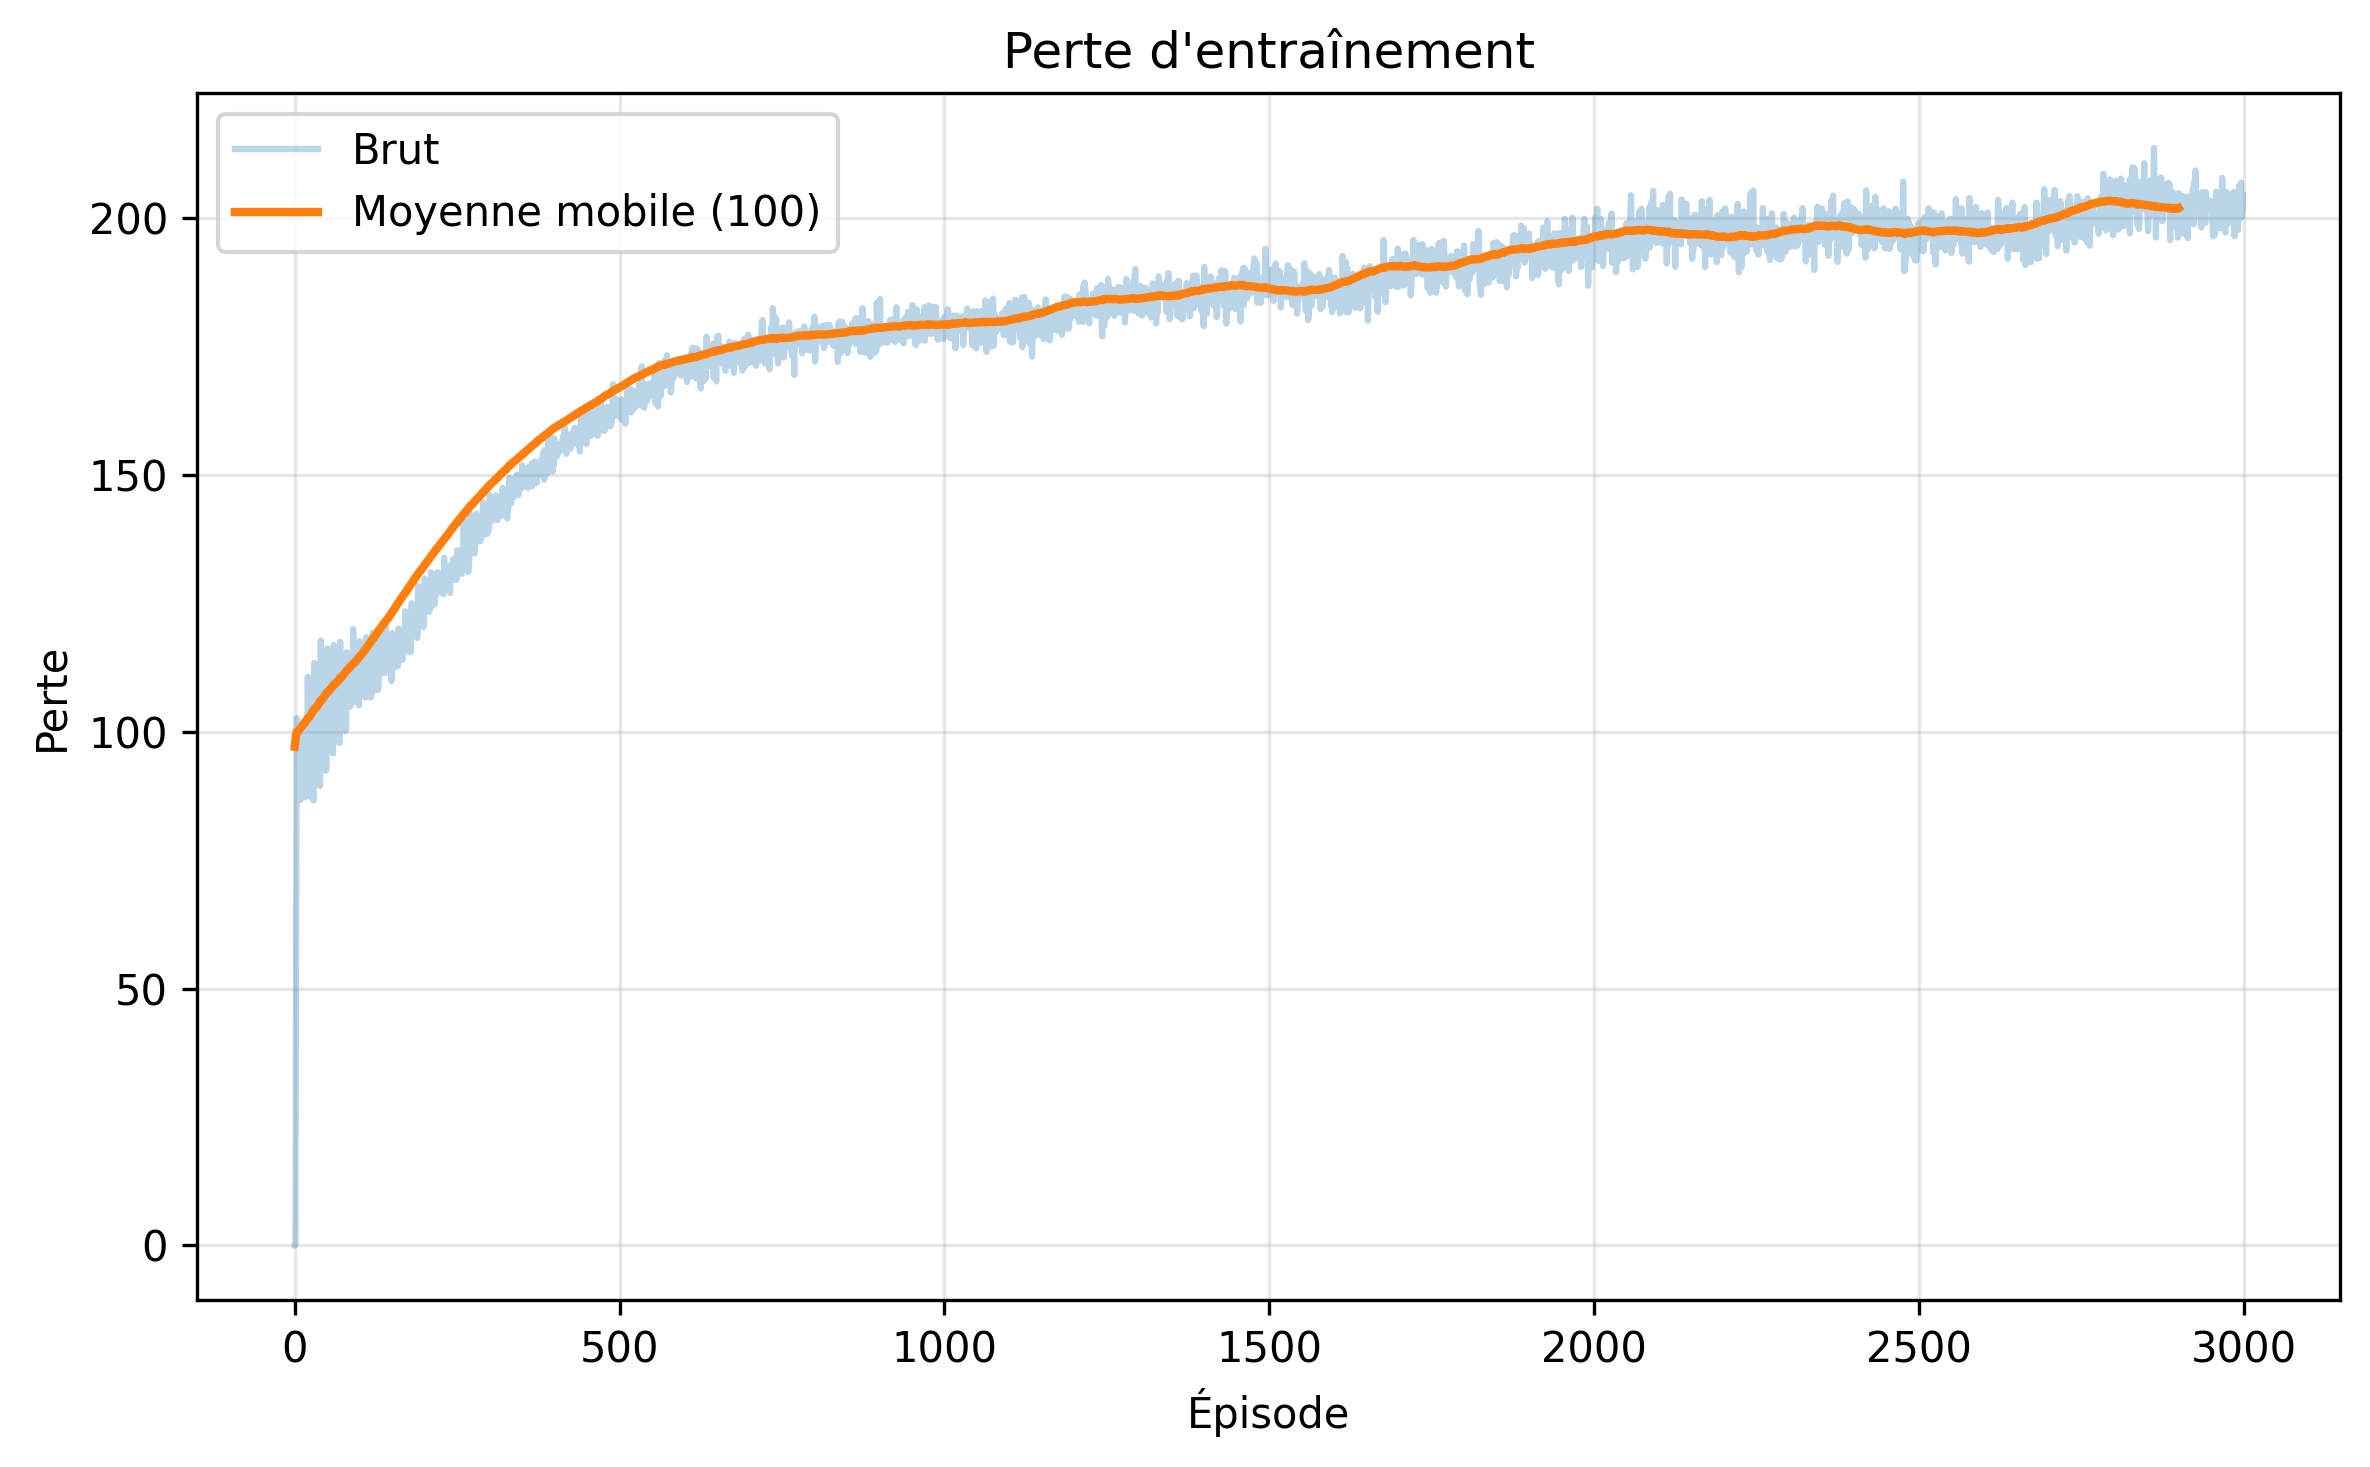
\includegraphics[width=\textwidth]{images/validation/training/03_perte_entrainement.png}
		\caption{Évolution de la fonction de perte}
		\label{fig:loss}
	\end{subfigure}
	\hfill
	\begin{subfigure}[b]{0.48\textwidth}
		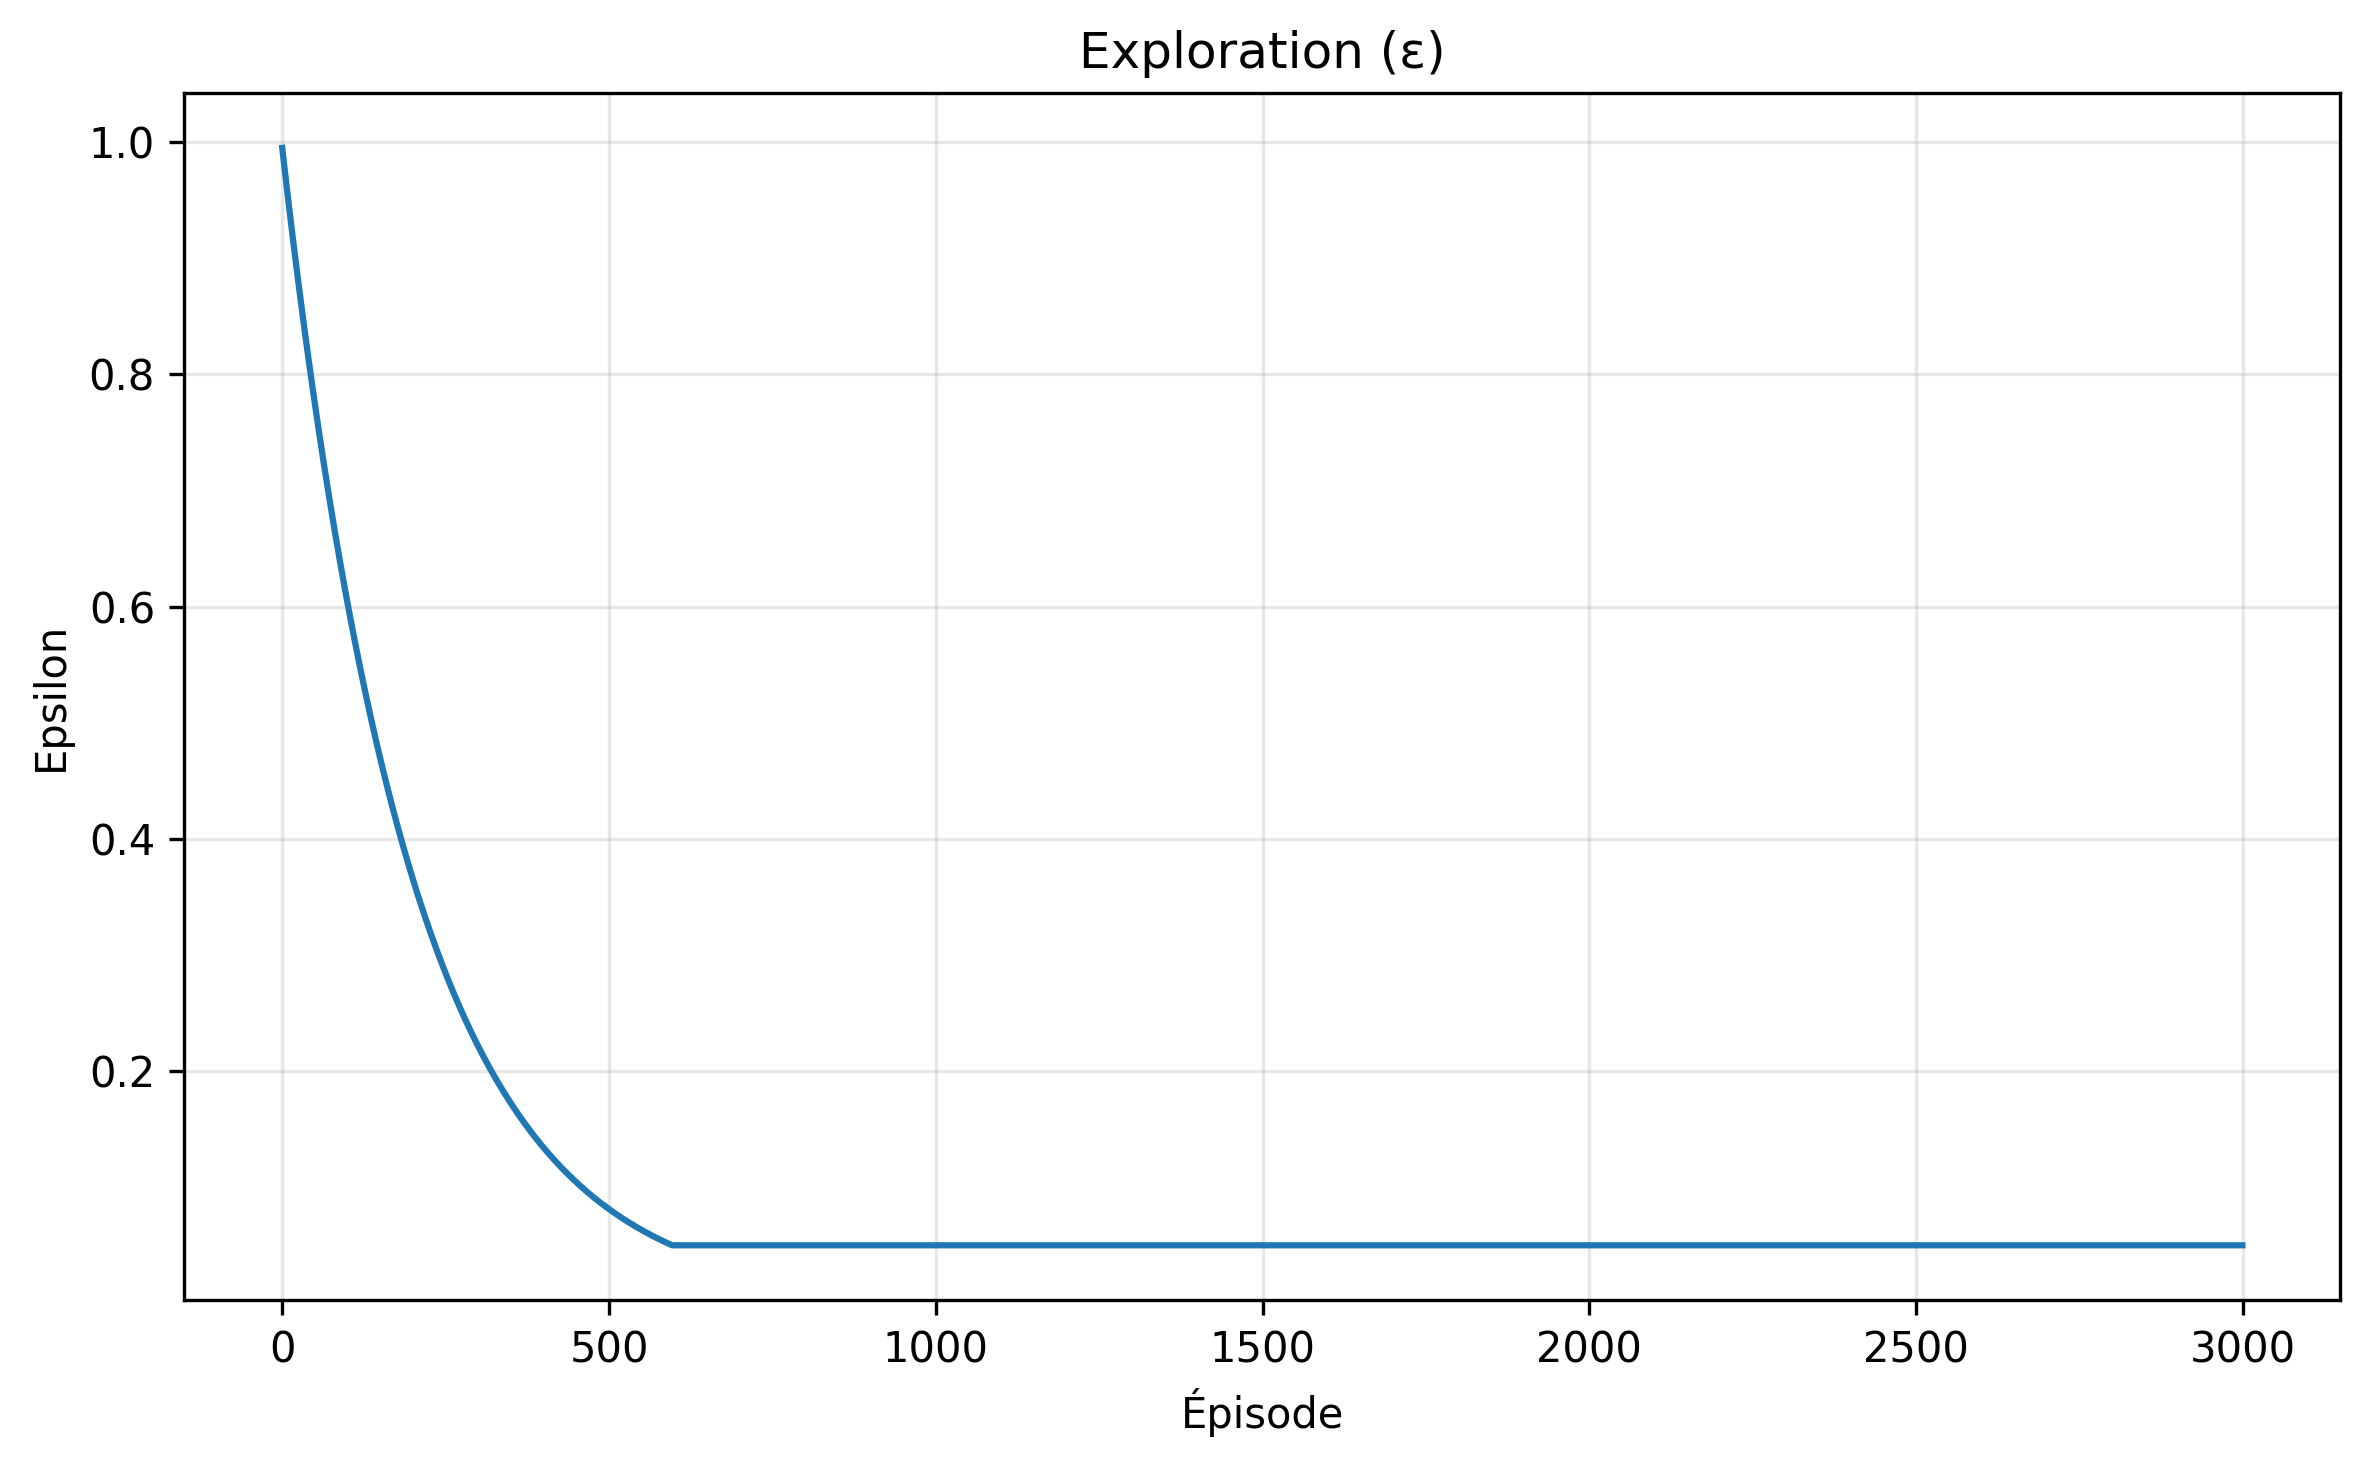
\includegraphics[width=\textwidth]{images/validation/training/05_epsilon.png}
		\caption{Décroissance de la stratégie $\epsilon$-greedy}
		\label{fig:epsilon}
	\end{subfigure}
	\caption{Courbes d'apprentissage de l'agent DDQN}
	\label{fig:training_curves}
\end{figure}


\section{Conclusion}
\label{sec:conclusion-ddqn}

Ce chapitre a posé les fondations théoriques et pratiques de notre approche d'optimisation par apprentissage par renforcement pour les réseaux LR-FHSS. En formulant le problème comme un processus de décision markovien, nous avons défini un cadre pour l'apprentissage d'une politique de transmission adaptative. Le chapitre suivant est entièrement dédié à l'évaluation expérimentale de cette solution.